%\documentclass[handout]{beamer}
\documentclass[aspectratio=169]{beamer}
\usepackage{etex} % fixes new-dimension error

\usetheme{metropolis}
\usepackage{appendixnumberbeamer}

% Base colors (from metropolis theme)
\definecolor{metDarkBrown}{HTML}{604c38}
\definecolor{metDarkTeal}{HTML}{23373b}
\definecolor{metLightBrown}{HTML}{EB811B}
\definecolor{metLightGreen}{HTML}{14B03D}

 

\metroset{numbering=fraction,progressbar=frametitle}

% \setbeamercolor*{structure}{fg=blue!80!black}
\setbeamercolor*{structure}{fg=metLightGreen}

% % \definecolor{MainColour}{rgb}{0., 0.25, 0.8}
% \colorlet{MainColour}{blue!50!black}
% \colorlet{BgColour}{blue!10}
% \colorlet{BarColour}{blue!50!black}


% %\usetheme{CambridgeUS}%{Copenhagen}%{Frankfurt}%{Singapore}%{CambridgeUS}
% \usecolortheme[named=MainColour]{structure} 
% \useoutertheme[subsection=false]{miniframes}
% \useinnertheme{circles}
% %\useinnertheme[shadow=false]{rounded}
% \setbeamertemplate{blocks}[rounded][shadow=false]

% \setbeamercovered{transparent} 
% \setbeamertemplate{navigation symbols}{} %Remove navigation bar
% \setbeamertemplate{footline}[frame number] % add page number
% \setbeamercolor{postit}{fg=MainColour,bg=BgColour}
% \setbeamercolor{structure}{bg=black!10}
% %\setbeamercolor{palette primary}{use=structure,fg=red,bg=green}
% %\setbeamercolor{palette secondary}{use=structure,fg=red!75!black,bg=green}
% \setbeamercolor{palette tertiary}{use=structure,bg=BarColour,fg=white}
% %\setbeamercolor{palette quaternary}{fg=black,bg=green}
% %\setbeamercolor{normal text}{fg=black,bg=white}
% %\setbeamercolor{block title alerted}{fg=red,bg=green}
% %\setbeamercolor{block title example}{bg=black!10,fg=green}
\setbeamercolor{block body}{bg=black!5}

% \setbeamercolor{block title alerted}{bg=red!25}
% \setbeamercolor{block body alerted}{bg=red!10}

% \setbeamercolor{block title example}{bg={rgb:green,2;black,1;white,5}}
\setbeamercolor{block body example}{bg={rgb:green,2;black,1;white,20}}
\setbeamercolor{block body alerted}{bg={metLightBrown!25}}

% \setbeamertemplate{itemize item}{\color{black!10}$\blacksquare$}
\setbeamercolor{itemize item}{fg=metDarkTeal}
\setbeamercolor{itemize subitem}{fg=metDarkTeal}

\setbeamercolor{graybc}{fg=black,bg=black!10}
\newcommand{\myblock}[1]{\begin{beamercolorbox}[dp=1ex,center,rounded=true]%
  {graybc} {\large \textbf{#1}} \end{beamercolorbox}}%


\usepackage{etex} % fixes new-dimension error
\usepackage{lmodern} % fixes warnings
\usepackage{textcomp}% fixes warnings

\usepackage{graphicx,amsmath}
\usepackage{stmaryrd} % cf. interleave
%\usepackage{./macros/myisolatin1}
%\usepackage{./macros/prooftree}
\usepackage{alltt}
%\usepackage{./macros/circle}
\usepackage{listings}
\usepackage{relsize} % relative size fonts
\usepackage[normalem]{ulem} % strikethrough text (with \sout{.})
\usepackage{tikz}
\usetikzlibrary{%
  positioning
 ,patterns
 ,arrows
 ,automata
 ,calc
 ,shapes
 ,fit
 ,fadings
 ,decorations.pathreplacing
 ,plotmarks
% ,pgfplots.groupplots
 ,decorations.markings
}
% \tikzset{shorten >=1pt,node distance=2cm,on grid,auto,initial text={},inner sep=2pt}
\tikzstyle{aut}=[shorten >=1pt,node distance=2cm,on grid,auto,initial text={},inner sep=2pt]
\tikzstyle{st}=[circle,draw=black,fill=black!10,inner sep=3pt]
\tikzstyle{sst}=[rectangle,draw=none,fill=none,inner sep=3pt]
\tikzstyle{final}=[accepting]
\usepackage[normalem]{ulem} % striking out text with \sout{...}
\usepackage{xspace}

\usepackage{transparent}

% Nicer TT fonts
\usepackage[scaled=.83]{beramono}
\usepackage[T1]{fontenc}




%------ using eurosym -------------------------------------------------------
\usepackage{eurosym}
\def\inh#1{\mbox{\small\euro}_{#1}}
\def\eith#1#2{\mathopen{[}#1 \ ,#2\mathclose{]}}

%------ using xy ------------------------------------------------------------
\usepackage[all]{xy}
%\def\larrow#1#2#3{\xymatrix{ #3 & #1 \ar[l] _-{#2} }}
\def\larrow#1#2#3{\xymatrix{ #3 & #1 \ar[l] _--{#2} }}
\def\rarrow#1#2#3{\xymatrix{ #1 \ar[r]^-{#2} & #3 }}
\def\arLaw#1#2#3#4#5{
\xymatrix{
        #1      \ar@/^1pc/[rr]^-{#4} &
        #5 &
        #2      \ar@/^1pc/[ll]^-{#3}
}}
\def\arLeq#1#2#3#4{\arLaw{#1}{#2}{#3}{#4}\leq}
%------ using pstricks (rnode etc) ------------------------------------------
%\usepackage{pstricks,pst-node,pst-text,pst-3d}
%------ using color ---------------------------------------------------------
%\newrgbcolor{goldenrod}{.80392 .60784 .11373}
%\newrgbcolor{darkgoldenrod}{.5451 .39608 .03137}
%\newrgbcolor{brown}{.15 .15 .15}
%\newrgbcolor{darkolivegreen}{.33333 .41961 .18431}
\definecolor{goldenrod}{rgb}{.80392,.60784,.11373}
\definecolor{darkgoldenrod}{rgb}{.5451,.39608,.03137}
\definecolor{brown}{rgb}{.15,.15,.15}
\definecolor{darkolivegreen}{rgb}{.33333,.41961,.18431}
\definecolor{darkgreen}{rgb}{0,0.6,0}
%
%
%\def\gold#1{{\textcolor{goldenrod}{#1}}}
%\def\brw#1{{\brown #1}}
%%\def\gre#1{{\green #1}}

\def\dgold#1{{\textcolor{darkgoldenrod}{#1}}}
\def\dkb#1{\textcolor{blue}{#1}}
\def\tdkb#1{\textbf{\textcolor{darkblue}{#1}}}
\def\gre#1{\textcolor{darkolivegreen}{#1}}
\def\gry#1{\textcolor{gray}{#1}}
\def\rdb#1{\textcolor{red}{#1}}

\definecolor{myGray}{gray}{0.85}
\newcommand{\red}[1]{\textcolor{red!80!black}{#1}\xspace}
\newcommand{\blue}[1]{\textcolor{blue}{#1}\xspace}
\newcommand{\gold}[1]{\textcolor{darkgoldenrod}{#1}\xspace}
\newcommand{\gray}[1]{\textcolor{myGray}{#1}\xspace}
\def\laplace#1#2{*\txt{\mbox{ \fcolorbox{black}{myGray}{$\begin{array}{c}\mbox{#1}\\\\#2\\\\\end{array}$} }}}
\newenvironment{bluein}{\blue}{\black\hskip -2.5pt}

%------ Setting lecture info ----------------------------------------------

\newcounter{lectureID}
\stepcounter{lectureID}
\newcommand{\getLecture}{\arabic{lectureID}\xspace}
\newcommand{\setLectureBasic}[1]{
  \title{
    #1
    }
  \author{David Pereira \and Jos\'{e} Proen\c{c}a \and Eduardo Tovar}
  \institute{CISTER -- ISEP \\ Porto, Portugal \flushright\url{https://cister-labs.github.io/fvoca2122}}
  \date{FVOCA 2021/2022\\Formal Verification of Critical Applications}
}
\newcommand{\setLecture}[2]{\setcounter{lectureID}{#1}\setLectureBasic{#2}}


\newcounter{cExercise}
\newcommand{\exercise}{\stepcounter{cExercise}Ex.\,\arabic{lectureID}.\arabic{cExercise}:\xspace}
\newcommand{\exerciseBack}{\addtocounter{cExercise}{-1}}
\newcommand{\exerciseAdd}{\stepcounter{cExercise}}
\newcommand{\doExercise}[3][0mm]{\begin{exampleblock}{\exercise #2}\wrap{\rule{0pt}{#1}}#3\end{exampleblock}}
\newcommand{\doSimpleExercise}[2][0mm]{\begin{exampleblock}{}\wrap{\rule{0pt}{#1}}\structure{\textbf{\exercise} #2}\end{exampleblock}}


%------ contexts  ---------------------------------------------------------
\newcounter{prg}
\newenvironment{prg}[1]{\refstepcounter{prg}
\noindent
\textsc{\textbf{\arabic{prg}.}} \textsc{#1} } 
{\vspace{5mm}}

\newenvironment{sprg}[1]{
\noindent
\textsc{#1} }
{\vspace{3mm}}

\newcommand\blfootnote[1]{%
  \begingroup
  \renewcommand\thefootnote{}\footnote{#1}%
  \addtocounter{footnote}{-1}%
  \endgroup
}


\newtheorem{defi}{Defini\cao}[section]
\newtheorem{defi*}{Defini\cao}
\newtheorem{lema*}{Lema}
\newenvironment{lsbcom}
      {\footnotesize  \hrule ~\\ ~\\ {\bf \sc Nota:} }
      {\hrule  ~\\ ~\\  \normalsize}
      
\newenvironment{lsbcomi}
      {\footnotesize  \hrule ~\\ ~\\ {\bf \sc Note:} }
      {\hrule  ~\\ ~\\  \normalsize}
      
\newcommand{\fimdemo}{%
\raisebox{1.7mm}{\framebox[2mm]{\rule{0mm}{0mm}}}%
\hspace{-1.55mm}%
\rule{2mm}{0.5mm}%
\hspace{-0.45mm}%
\rule{0.5mm}{2mm}%
}

\newenvironment{intf}%
     {\traco}
    {\par \nopagebreak  \traco }
\newenvironment{demo}%
     {\vspace{-5mm}\noindent {\bf Prova:}}%
    {\par \nopagebreak  \noindent \fimdemo \vspace{3mm} }
\newenvironment{demoi}%
     {\vspace{-5mm}\noindent {\bf Proof:}}%
    {\par \nopagebreak  \noindent \fimdemo \vspace{3mm} }

\long\def\CUT#1{\relax}
\def\jnowarning#1{\typeout{Warning: #1 - document page [\thepage]}}

\newenvironment{slide}[1]{\begin{frame}\frametitle{#1}}{\end{frame}}
\long\def\marginproof#1#2{
\begin{slide}{Comments}
\footnotesize Proof of #1:\\\tiny#2
\end{slide}}

\long\def\margincomment#1{
\begin{slide}{Comments}
\footnotesize #1
\end{slide}}

\long\def\marginproof#1#2{\relax}
\long\def\margincomment#1{\relax}

\def\caixa#1{\medskip
  \begin{center}
  \fbox{\begin{minipage}{0.9\textwidth}\protect{#1}\end{minipage}}
  \end{center}}
  
  \def\caixam#1{\medskip
  \begin{center}
  \fbox{\begin{minipage}{0.9\textwidth}\protect{\vspace{-5mm}#1\vspace{-5mm}}\end{minipage}}
  \end{center}}
  
   \def\caixamm#1{\medskip
  \begin{center}
  \fbox{\begin{minipage}{0.9\textwidth}\protect{\vspace{-5mm}#1}\end{minipage}}
  \end{center}}

  
  \def\caixaaa#1{\medskip
  \begin{center}
  \fbox{\begin{minipage}{0.95\textwidth}\protect{#1}\end{minipage}}
  \end{center}}

\newcommand{\caixapeq}[2][0.71]{\medskip
  \fbox{\begin{minipage}{#1\textwidth}\protect{#2}\end{minipage}}}
  
  \def\caixapeqq#1{\medskip
  \fbox{\begin{minipage}{0.85\textwidth}\protect{#1}\end{minipage}}}
  
  \def\caixamin#1{
   \begin{center}
  \fbox{\begin{minipage}{0.70\textwidth}\protect{\vspace{-5mm}#1}\end{minipage}}
  \end{center}}


\def\endprf{\begin{flushright} $\Box$ \end{flushright} \vspace{3mm}}

%------ common jno, lab  ---------------------------------------------------------
%------------
\def\wider#1{~ #1 ~}
\def\altx#1#2{\mathopen{[}#1 \ ,#2\mathclose{]}}
\def\X{\end{document}}
\def\EXIT{ \bibliographystyle{plain} \bibliography{/Users/jno/share/texinputs/jno} \end{document}}
%------------
\def\fdep#1#2#3{#1 \mathbin{\stackrel{#2}{\rightarrow\/}} #3}
\def\lift#1{\stackrel.{#1}}
\newcommand{\N}{\mathbb{N}}
\newcommand{\Z}{\mathbb{Z}}
%\def\N{I\!\!N}                             % Nat numbers
%\def\Z{Z\!\!\!Z}                           % Integers
\def\real{I\!\!R}                           % Integers

\def\name#1{\makebox[15ex][l]{\emph{#1:}} &&}
\let\kons=\underline
\def\selup#1#2#3{#3^{#1}_{#2}}
\def\plus{\mathbin{\dagger}}
\def\asor{\mathbin{|}}                    % A | B
\def\enlist#1{\mathopen{[}#1\mathclose{]}} % [a,b,...z]
\def\from{\mathbin{\leftarrow}}
\def\listdef#1#2{\enlist{ ~ #1 \asor #2 \,}} % < f(x) | x <- l>
\def\into{\mathbin{\rightarrow}}
\let\seqdef=\listdef
\def\Seq#1{{#1}^{\star}}                 % X*
\def\f{\fun F}
\def\fuc#1{\mathsf {#1}}
\def\fun#1{\mathsf {#1}}
\def\g{\fun G}
\def\ff#1{\ap\f{#1}}
\def\gg#1{\ap\g{#1}}
\def\hfilleqn#1#2{\hfill$#1\arrayin{#2}$\hfill~}
\def\enset#1{\mathopen{ \{ }#1\mathclose{ \} }} % {a,b,...z}
\newcommand{\set}[1]{\left\{ #1 \right\}} % {a,b,...z}
\def\mcond#1#2#3{#1 \rightarrow #2,#3}
\def\bang{{!}}
\def\ap#1#2{#1\,#2}
\def\pow#1{\ap{{\cal P}}{(#1)}}           \def\pow#1{{\cal P}#1} % P(X) redefined
\def\unary#1#2{\def\arg{#2}\def\omisso{}\ifx\arg\omisso{\textsf{#1}}\else\ap{\textsf{#1}}{#2}\fi}
\def\card#1{\unary{card}{#1}}             % card 
\def\ker#1{\unary{ker}{#1}}  
\def\img#1{\unary{img}{#1}}
\def\st{\dot}
\def\len#1{\unary{len}{#1}}
\def\inds#1{\unary{inds}{#1}}
\def\dom#1{\unary{$\delta$}{#1}}
\def\rng#1{\unary{$\rho$}{#1}}
\let\ran=\rng
\def\issat{\mathbin\vdash}
\def\post#1{\hbox{post-}{#1}}              % post-#1
\def\pre#1{\hbox{pre-}{#1}}                % pre-#1
\def\presat{\mathbin{\issat_{pre}}}
\def\postsat{\mathbin{\issat_{post}}}
\def\laplace#1#2{*\txt{\fbox{$\begin{array}{c}\mbox{#1}\\\\#2\\\\\end{array}$}}}
\def\PF{{\cal PF}}
\def\ler#1{{\red \em [ read: #1]}}

\def\proj#1{\pi_{#1}}
%\def\deff{\stackrel{\rm def}{=}}          % Function definition symbol
\def\deff{\, :=\, }          % Function definition symbol
\def\setdef#1#2{\mathopen{\{} #1 \asor #2 \mathclose{\}}}
\def\asor{\mathbin{|}}                    % A | B
\def\p#1{\pi_{#1}}
\def\mvdep#1#2#3{#1 \mathbin{\stackrel{\rule[-.8ex]{0pt}{0pt}#2}{\rightharpoonup\hskip-1.5ex\rightharpoonup\/}} #3}
\def\gmvdep#1#2#3#4{#1 \mathbin{\stackrel{\rule[-.8ex]{0pt}{0pt}#2}{\rightharpoonup\hskip-1.5ex\rightharpoonup_{#4}\/}} #3}
\def\sshylo#1#2{\mean{~#1,#2~}}
\def\cata#1#2{\mathopen{(\!|}#1\mathclose{|\!)}_{{\fun #2}}}
\def\split#1#2{\const{#1,#2}}
\def\tuple#1{\mathopen{\langle}#1\mathclose{\rangle}} % <a,b,...z>
\def\divides{\mathbin{\setminus}}
\def\rdiv{\mathbin{\setminus}}
\def\ldiv{\mathbin{/}}
\def\true{\mathsf{true}}
\def\mean#1{\mathopen{[\![}#1\mathclose{]\!]}}
\def\false{\mathsf{false}}
\newenvironment{lcbr}{\left\{\begin{array}{l}}{\end{array}\right.}
\def\rcb#1#2#3#4{\def\nothing{}\def\range{#3}\mathopen{\langle}#1 \ #2 \ \ifx\range\nothing::\else: \ #3 :\fi \ #4\mathclose{\rangle}}

\def\rcbVdm#1#2#3#4{#1 \ #2 \ � #4}
\def\deffVdm{\mathbin{\raisebox{.2em}{\tiny \ \underline{$\mathchar"3234$} \ }}}
\def\mapVdm#1#2{#1 \mathbin{\tilde{\rightarrow}} #2}

\def\const#1{\mathopen{\langle}#1\mathclose{\rangle}} % <a,b,...z>
\def\comp{\mathbin{\cdot}}
\def\implied{\mathbin\Leftarrow}
\def\implies{\mathbin{\Rightarrow}}
\def\arrayin#1{\begin{array}{rcl}#1\end{array}}
\def\xarrayin#1{\begin{array}{cccccc}#1\end{array}}
\def\aspas#1{``#1''}
\def\ap#1#2{#1\,#2}
\def\unary#1#2{\def\arg{#2}\def\omisso{}\ifx\arg\omisso{\textsf{#1}}\else\ap{\textsf{#1}}{#2}\fi}
\def\card#1{\unary{card}{#1}}             % card x
\def\ker#1{\unary{ker}{#1}}  
\def\img#1{\unary{img}{#1}}
\def\ijust#1#2{&#1& \rule{2em}{0pt}  \{ \mbox{\rule[-.5em]{0pt}{1.2em} \footnotesize #2 \/} \}  \nonumber\\ && }
\def\just#1#2{\\\ijust{#1}{#2}}

\def\crflx#1{\Phi_{#1}}
\def\qcomp{\mathbin\bullet}
\def\xlarrow#1#2#3{\larrow{#3}{#2}{#1}} 
%\def\equiv{\Leftrightarrow}
\def\longlarrow#1#2#3{\xymatrix{ #3 && #1 \ar[ll] _-{#2} }}
%------------

%------  lsb  ---------------------------------------------------------

\def\drawit{\nccurve[angleA=-30,angleB=-150]{->}{NA}{NB}}

\def\cnext#1{\Circle_{#1}}
\def\clast#1{\Circle[f]_{#1}}
\def\calfut#1{\square_{#1}}

\def\mdepth#1{\mathsf{md}\, #1}

\def\always{\boxempty}
\def\eventual{\Diamond}
\def\nexts{\bigcirc}
\def\until{\mathbin{\mathcal U}}


\def\setFontSize#1{\gdef\currentFontSize{#1}\fontfamily{phv}\fontsize\currentFontSize\currentFontSize\selectfont}
\def\greybox#1{*\txt{\mbox{\fcolorbox{black}{myGray}{\mbox(40,15){#1}}}}}
\def\funbox#1{*\txt{\fcolorbox{white}{myGray}{\makebox(40,15){\black $#1$}}}}
\def\condition#1{*\txt{\fontfamily{phv}\fontsize\currentFontSize\currentFontSize\selectfont\pscirclebox[linecolor=white]{$#1$}}}
\def\checkpoint{*\txt{\pscirclebox*{}}}
\def\state{*\txt{\ovalnode[fillstyle=solid,fillcolor=red]{State}{\black Internal state}}}
\def\thing#1{$\bullet$ \rule{0pt}{.7cm} & \fcolorbox{black}{myGray}{#1}}

\def\const#1{\mathopen{\langle}#1\mathclose{\rangle}} % <a,b,...z>
\def\funbox#1{*\txt{\fcolorbox{white}{gray}{\makebox(40,15){\black $#1$}}}}
\def\pair#1{\const{#1}}
\def\bim{\fuc{B}}
%\def\abim#1{\bim\, #1}
\def\abim#1{\aapf{\bim}{#1}}
\def\bimm#1{\bim #1}
\def\iso{\cong}
\def\niso{\ncong}
\def\qcom{\mathbin{\boldsymbol{;}}}
\def\id{\fuc{id}}

\def\ainv#1{\overline{#1}}

\def\rsrt{\tau_{r}}   % right and left strength
\def\rsrtp#1{\tau_{r_{#1}}}   % right and left strength
\def\lsrt{\tau_{l}}

\def\igual{\mathbin{=}}
\def\dimp{\mathbin{\Leftrightarrow}}
\def\imp{\mathbin{\Rightarrow}}
\def\dimpp{\mathbin{\leftrightarrow}}
\def\impp{\mathbin{\rightarrow}}
\def\rimp{\mathbin{\Leftarrow}}
\def\limp{\mathbin{\multimap}}

\newcommand{\sse}{\mathbin{\, \operatorname{\textsf{iff}} \,}}
\def\e{\mathbin{\wedge}}
\def\ou{\mathbin{\vee}}

\def\aconv#1{#1^{\circ}} 
\newcommand{\fdec}[3]{#1: #2 \longrightarrow  #3}
\newcommand{\fdecf}[3]{#1: #2 \longrightarrow #3}
\newcommand{\fdef}[2]{#1\;=\; #2}

\newcommand{\adec}[3]{#1 \stackrel{#2}\longrightarrow #3}
\newcommand{\fblockf}[5]{
\begin{eqnarray*}
#1&\! \! \!: \!\! \!& #2 \longrightarrow #3\\
#1 & \! \!\! #4\, = \!\!\!& #5
\end{eqnarray*}
}

\newcommand{\sos}[3]{#3 \stackrel{#2}{\longleftarrow} #1}
\def\setcat{{\sf Set}}
\def\relcat{{\sf Rel}}
\def\parcat{{\sf Par}}
\def\predcat{{\sf Pred}}
\def\ordcat{{\sf Ord}}

\def\dois{\ensuremath{\boldsymbol{2}}}
\def\abv{\stackrel{\rm abv}{=}}
\def\sana#1{\mathopen{[\!(}#1\mathclose{)\!]}}
\def\deff{\triangleq} 
\def\pint{\mathbin{\interleave}}



% Fev 2010

\def\oculos{\mathbf{\bigcirc\!\! \frown\!\! \bigcirc}}
\def\ferramentas{\stackrel{\mathbf{\doublecap}}{\bigbox\!\!\bigbox}}
%\def\Act{\cal{N}}
\def\Act{N}

\def\vec#1{\Tilde{#1}}
\def\free#1{\textsf{free}(#1)}
\def\subs#1#2#3{\enset{#1/#2}\, #3}

\def\tim{\fuc{T}}
\def\att{\fuc{at}}
\def\md{\fuc{m}}

\def\bh#1#2{\apf{\ana{#1}}{#2}}

\def\apf#1#2{#1\; #2}                   % func applic no () -- f a
\def\appf#1#2{(#1\; #2)}                   % func applic with () -- (f a)
\def\aapf#1#2{#1 #2}                   % func applic no () -- f a

\def\aappf#1#2{(#1 #2)}                   % func applic with () -- (f a)
\def\appff#1#2{#1 (#2)}                   % func applic with () -- f(a)
%\def\ana#1#2{\mathopen{[\!(}#1\mathclose{)\!]}_{#2}}
%\def\ana#1#2{\mathopen{[\!(}#1\mathclose{)\!]}_{\fun #2}}
\def\ana#1{\mathopen{[\!(}#1\mathclose{)\!]}}
\def\sana#1{\mathopen{[\!(}#1\mathclose{)\!]}}

\def\iid#1{\id_{#1}}                     %  identitade default
\def\id{\mathbin{\fuc{id}}}    

\def\atim#1{\aapf{\tim}{#1}}
\def\final#1{\omega_{#1}}
\def\initial#1{\alpha_{#1}}

\def\ialg#1{\mu_{#1}}
\def\fcoalg#1{\nu_{#1}}
\def\hdd{\fun{hd}}
\def\tll{\fun{tl}}
\def\mrg{\fun{merge}}
\def\gnn{\fun{rep}}
\def\diag{\vartriangle}
\def\codiag{\triangledown}
\def\twist{\fun{twist}}
\def\swap{\fuc{s}}
\def\rtran#1{\stackrel{#1}{\longrightarrow}}
\def\rtrant#1{\stackrel{#1}{\longrightarrow}^{\raisebox{-4pt}{\scriptsize $*$}}}
\def\tran#1{\stackrel{#1}{\longrightarrow}}
\def\primertran#1{\stackrel{#1}{\longrightarrow'}}
\def\rra{\longrightarrow}
\def\dda{{\downarrow}}
\def\ppow{\ensuremath{\mathcal{P}}} 
\def\nx{\fun{next}}
\def\utran#1{\stackrel{#1}{\longrightarrow}}  % - a - > 
\def\reach#1{\stackrel{#1}{\longrightarrow}^*}

\newcommand{\blk}[1]{\mathbb{#1}}
\newcommand{\ger}[1]{\mathfrak{#1}}

\def\vs{\emph{vs}}
\def\ie{\emph{i.e.}}
\def\cf{\emph{cf.}}

\def\eg{\emph{e.g.}}

\def\PP{\blk{P}}

%------ CCS          -----------------------------------------%
\def\ppe{\mathbin{\vartriangleright}}
\def\kcomp{\mathbin{\boldsymbol{\bullet}}}
%\def\qcomp{\mathbin{\boldsymbol{;}}}
\def\ssp{\textsc{skip}}
\def\fim{\dagger}
%\def\ppe{\gg}
\def\cnil{\mathbf{0}}
\def\cpf#1#2{#1 . #2}                           % a.P
\def\cou#1#2{#1 \mathbin{+} #2}                 % P + Q
%\def\crt#1#2{\mathbin{#1 \setminus_{#2}}}       % P \ A
%\def\crtt#1#2{\mathbin{#1 \setminus\!\setminus_{#2}}}       % P \ A
%\def\crt#1#2{\mathsf{new}\, #2\;  #1}       % P \ A
\def\crt#1#2{#1 \backslash #2}       % P \ A
%\def\crn#1#2{\{#2\}\, #1}                  % P[f]

\def\crn#1#2{\mathbin{#1[#2]}}                  % P[f]
\def\couit#1#2{\Sigma_{#1}#2}                  %  + i=1,n
\def\cpar#1#2{#1 \mid #2}                       %  |
\def\ctpar#1#2{#1 \parallel #2}                       %  |
\def\cpars#1#2#3{#1 \mid_{#3} #2}               %  |S
\def\ffix#1#2{\underline{fix}~(#1\, =\, #2)}  % fix X
\def\fffix#1#2#3{\underline{fix}_{#1}~(#2\, =\, #3)}  % fix X
\def\tfix#1#2{\underline{\Tilde{fix}}~(\Tilde{#1}\, =\, \Tilde{#2})}  % fix X
%\def\ainv#1{\Bar{#1}}                   % ~ a
\def\ainv#1{\overline{#1}}                   % ~ a
\def\cif#1#2{\fuc{if}\, #1\, \fuc{then}\, #2}
\def\ccif#1#2#3{\fuc{if}\, #1\, \fuc{then}\, #2\, \fuc{else}\, #3}

\def\fres#1#2{#1 \restriction #2}                

\def\mean#1{\mathopen{[\![}#1\mathclose{]\!]}}
\def\llbracket{\mathopen{[\![}}
\def\rrbracket{\mathopen{]\!]}}

\def\cfree#1{\fuc{fn} (#1)}
\def\cbound#1{\fuc{bn} (#1)}
\def\anew#1{\overline{#1}\mathsf{new}\, } 
\def\transitatau{\rtran{\tau}}
\def\transitaa{\rtran{a}}


\def\cHat#1{{\cal T}(#1)}
\def\free#1{\textsf{free}(#1)}
\def\fuc#1{\textsf{#1}}
\def\subs#1#2#3{\enset{#1/#2}\, #3}
\def\PP{\blk{P}}
\def\PPf{\blk{P}_{\fim}}
\def\obs{\mathbin{\sim}}                     % P ~ Q
\def\nobs{\mathbin{\nsim}}                     % P ~ Q
\def\aobs{\mathbin{\approx}}                 % P ~ Q
\def\naobs{\mathbin{\not \approx}}                 % P ~ Q
\def\cobs{=}                                 % P = Q
\def\ssort#1{\blk{L}(#1)}                   % L()
\def\sysort#1{\blk{L}_s(#1)}                   % L()

\def\athen{\comp}
\def\PP{\blk{P}}

% 2015

\def\st{\mathbf{.}\,}
\def\laplace#1#2{*\txt{\mbox{ \fcolorbox{black}{myGray}{$\begin{array}{c}\mbox{#1}\\\\#2\\\\\end{array}$} }}}
\newcommand{\galois}[2]{#1\; \dashv\; #2}

\newcommand{\fddec}[3]{#1: #2 \longrightarrow  #3}

\def\mcrl{\textsf{mCRL2}}

\def\obs{\sim}
\def\eqm{\mathbin{\equiv}}                     
\def\noeqm{\mathbin{\not\!\equiv}}  
\newcommand{\flam}[2]{\lambda_{#1}\; .\; #2}
\def\existential#1#2{\exists_{#1}\;.\; #2}
\def\existencial#1#2{\exists_{#1}\;.\; #2}

\def\diam#1{\ensuremath{\langle #1 \rangle}}
\def\boxx#1{\ensuremath{[#1]}}
\def\pv#1#2{\langle #1 \rangle\, #2}
\def\nc#1#2{[#1]\, #2}
\def\pvo#1#2{\langle \! \! \! \langle #1 \rangle \! \! \! \rangle\, #2}
\def\nco#1#2{\llbracket #1 \rrbracket #2}
\def\cvg#1{\llbracket \downarrow \rrbracket #1}
\def\cvgr#1#2{\llbracket #1 \downarrow \rrbracket #2}
\def\cvgl#1#2{\llbracket \downarrow  #1 \rrbracket #2}
\def\cvglr#1#2{\llbracket \downarrow  #1 \downarrow \rrbracket #2}
\def\lfp#1#2{\mu {#1}\, .\, {#2}}
\def\lpf#1#2{\mu {#1}\, .\, {#2}}
\def\gfp#1#2{\nu {#1}\, .\, {#2}}
\def\gpf#1#2{\nu {#1}\, .\, {#2}}
\def\mset#1{\vvv #1 \vvv}
\def\vvv{\vert \! \vert}
\def\mnc#1{\vvv [#1] \vvv}
\def\mpv#1{\vvv \langle #1 \rangle \vvv}
\def\bcomp#1{#1^{\text{c}}}
\def\eqm{\mathbin{\simeq}}
\def\noeqm{\mathbin{\not\!\simeq}}
\def\universal#1#2{\forall_{#1}\; .\; #2}
\def\existential#1#2{\exists_{#1}\; .\; #2}
\def\oexistential#1#2{\exists^{1}_{#1}\; .\; #2}

\def\reach#1{\stackrel{#1}{\longrightarrow}^*}


\def\rra{\longrightarrow}

\def\Lg#1{\mathsf{Lang}(#1)}
\def\Tr#1{\mathsf{Tr}(#1)}

\def\PP{\blk{P}}

\def\paths#1{\mathsf{Paths}(#1)}
\def\Mcomma{\text{ ,}}
\def\Msemicolon{\text{ ;}}
\def\Mdot{\text{ .}}


%%%%%%%%%%%%%%%% NUNO reconf

\def\node#1{\ensuremath{\underline{#1}}}
\def\nameset{\ensuremath{\mathcal{I}}\xspace}
\def\endnameset{\ensuremath{\mathcal{E}}\xspace}
\def\nodeset{\ensuremath{\mathcal{N}}\xspace}
\def\portset{\ensuremath{\Sigma}\xspace}
\def\coordpatset{\ensuremath{\mathcal{P}}\xspace}
\def\logicmodel{\ensuremath{\mathcal{M}}\xspace}
\def\reconfset{\ensuremath{\mathcal{R}}\xspace}
\def\reconfoperationset{\ensuremath{\mathcal{O}}\xspace}
\def\channelset{\ensuremath{\mathcal{C}}\xspace}
\def\stateset{\ensuremath{\mathcal{S}}\xspace}
\def\typeset{\ensuremath{\mathcal{T}}\xspace}
\newcommand{\chanodesof}[2][\rho]{\ensuremath{\mathfrak{N}_{#1}^{#2}}\xspace}
\newcommand{\reconfop}{\ensuremath{\mathbin{\bullet}}}

\newcommand{\byreconfof}[1]{\ensuremath \stackrel{\rm #1}{\longleftarrow}}

\def\trans#1{\stackrel{#1}{\longrightarrow}}
\def\TS#1{\mathcal{G}(#1)}
\def\TSn#1{\mathcal{G}_{nodes}(#1)}


%%%%%%%%%%%%%%%%%%%%%%%%% ALEXANDRE
 \def\HHL{\mathcal{HHL}}
 
 \def\emskip{\vskip 1em}
 
 %%%%%%%%%%%%%%%%%%%%%% COMPONENTES NOV 2015
 \def\para{\mathbin{\boxtimes}}   % Mealy produto (sincrono)
\def\parc{\mathbin{\boxplus}}    % Mealy soma
\def\pars{\mathbin{\boxast}}     % Mealy misto
\def\shk#1#2{\bigl(#1\bigr)_{#2}}            % separated hook direita
\def\hk#1#2{#1\! \Lsh_{#2}}            % hook direita
\def\hkespaco#1#2{#1 \Lsh_{#2}}            % hook direita
%\def\feed#1{\Bigl( #1 \Bigr)\! \Lsh}            % hook direita
\def\feed#1{#1 \Lsh}            % hook direita
\def\kh#1#2{~_{#2}(#1)}           % hook esquerda

\def\flift#1{\ulcorner #1 \urcorner}           % funcoes embb
\def\singr#1{\lfloor #1 \rceil}

\def\pdiag{\bigtriangleup}      % diagonal em componentes
\def\pcodiag{\bigtriangledown}    % codiagonal em componentes

%\qcomp{\mathbin{\mathbf{;}}}
%\def\qcom#1#2{#1\qcomp#2}
%\def\sync{}  %d� problemas com o reotex.sty do Nuno Oliveria

 
 %%%%
 \def\SING{\ensuremath{\boldsymbol{1}}}
\def\ZERO{\ensuremath{\boldsymbol{0}}}

\def\ptran#1{\stackrel{#1}{\leadsto}}
\def\pptran#1#2{\stackrel{#1[#2]}{\leadsto}}

\def\bblue#1{\dkb{#1}}
\def\ctt#1{\underline{#1}}    
\def\lvazio{\fuc{nil}}   
\def\lcons{\mathbin{\fuc{cons}}} 
\def\either#1#2{[#1,#2]}
\def\att{\fun{at}}
\def\hd#1{\mathbin{\fuc{hd}} \, {#1}}              % hd x
\def\tl#1{\mathbin{\fuc{tl}} \, {#1}}   
\def\hdd{\mathbin{\fuc{hd}}}              % hd x
\def\tll{\mathbin{\fuc{tl}}}              % hd x\def\nnat{\blk{N}}
\def\rreal{\blk{R}}
\def\nnat{\blk{N}}
\def\vtran#1#2#3{#1\downarrow_{#3} #2 }
\def\labtran#1#2{~_{#1}\!\stackrel{#2}{\longleftarrow\, }}
\def\rabtran#1#2{\stackrel{#2}{\longrightarrow}_{#1}\, }
\def\excp#1{#1 + \SING}
\def\usplit#1#2{\langle #1, #2 \rangle}
\def\nnx{\fun{nx}}
\def\nxc{\ainv{\fun{nx}}}
%\def\ct{\fun{ct}}
%\def\ctc{\ainv{\fun{ct}}}
%\def\ini{\fun{ini}}
\def\nil{\underline{\fun{nil}}}
\def\att{\fun{at}}
\def\nx{\fun{next}}
\def\md{\fun{m}}
\def\acc{\ainv{\fun{ac}}}
\def\ac{\fun{ac}}
\newcommand{\mcar}[3]{(#1\, \rightarrow\, #2, \,   #3)}
\def\distr{\fuc{dr}}
\def\distl{\fuc{dl}}
\def\hdi#1{\mathbin{\fuc{last}} \, {#1}}              % hd x
\def\tli#1{\mathbin{\fuc{blast}} \, {#1}} 
\def\ip#1{\iota_{#1}}
\def\apf#1#2{#1\; #2}   
\def\m{\fuc{M}}

\def\onefuc{\fuc{Id}}
\def\triple#1{\const{#1}}
\def\kcomp{\mathbin{\boldsymbol{\bullet}}}  
 
\def\ntarrow{\Longrightarrow}
\newcommand{\ntdec}[3]{#1: #2 \ntarrow #3}
\def\ntiso{\stackrel{\iso}{\ntarrow}}

\def\rsrt{\tau_{r}}   % right and left strength
\def\rsrtp#1{\tau_{r_{#1}}}   % right and left strength
\def\lsrt{\tau_{l}}
\def\lsrtp#1{\tau_{l_{#1}}}   % right and left strength
\def\deltab{\delta}
\def\rpd{\delta_{r}}   % strength combination
\def\rpdp#1{\delta{r_{#1}}}
\def\lpd{\delta_{l}}
\def\ltrocam{\fuc{xl}_{+}}  % \assoc inv . \swap . \assoc
\def\rtrocam{\fuc{xr}_{+}}  
\def\dtrocam{\fuc{m}_{+}}  
\def\ltroca{\fuc{xl}}  % \assoc inv . \swap . \assoc
\def\rtroca{\fuc{xr}}  
\def\dtroca{\fuc{m}}  
\def\troca{\fuc{x}}  
\def\cat#1{{\sf #1}}
\def\flift#1{\ulcorner #1 \urcorner} 
\def\PR{\cat{Cp}}
\def\PRSp{\cat{Cp}_{Sp}}
\def\prcat#1{{\sf Cp_{#1}}}
%\newcommand{\prhom}[2]{\PR_{\bim}(#1, #2)}
\newcommand{\prhom}[2]{\PR(#1, #2)}
%\newcommand{\prhoms}[2]{\PR_{\bim}(#1, #2)_{Sp}}
\newcommand{\prhoms}[2]{\PR(#1, #2)_{Sp}}
\def\cid#1{\fuc{copy}_{#1}} 
\def\bismp#1{\sim{#1}}
\def\bism{\mathbin{\sim}}
\def\nbism{\overset{\bullet}{\sim}}
\def\nobism{\mathbin{\not\!\sim}}
\def\nilc{\fuc{nil}}
\def\idle{\fuc{idle}}
\def\inert#1{\fuc{inert}_{#1}}
\def\zerol{\fuc{zl}}
\def\zeror{\fuc{zr}}
\def\distr{\fuc{dr}}
\def\distl{\fuc{dl}}
\def\assoc{\fuc{a}}
\def\assocs{\fuc{a_*}}
\def\assocm{\fuc{a_+}}
\def\swap{\fuc{s}}
\def\swaps{\fuc{s_*}}
\def\swapm{\fuc{s_+}}
\def\lunit{\fuc{l}}
\def\runit{\fuc{r}}
\def\lunits{\fuc{l_*}}
\def\runits{\fuc{r_*}}
\def\lunitm{\fuc{l_+}}
\def\runitm{\fuc{r_+}}
\def\ana#1#2{\mathopen{[\!(}#1\mathclose{)\!]}_{#2}}
\def\sana#1{\mathopen{[\!(}#1\mathclose{)\!]}}
\def\bh#1#2{\apf{\ana{#1}}{#2}}
\def\BH{\cat{Bh}}
\def\diag{\vartriangle}
\def\codiag{\triangledown}
\def\psplit#1#2{\mathopen{\langle}#1, #2\mathclose{\rangle}}
\def\flift#1{\ulcorner #1 \urcorner} 
\def\rpdp#1{\delta{r_{#1}}}
\def\lpd{\delta_{l}}
%\def\lpdp#1{\lpd_{#1}}
\def\lpdp#1{\delta{l_{#1}}}

\def\bunit#1{\eta_{#1}}   % monad unit
\def\bmul#1{\mu_{#1}}   % monad multi

\def\bag#1{\fuc{Bag}_{#1}}

\newcommand{\MH}{\mathcal{H}}
\newcommand{\M}{M}
\newcommand{\Rz}{\textsc{T}}
\newcommand{\docircrlh}[2]{%
  \ooalign{$#1\rightarrow$\cr\hfil$#1\comp$\hfil\cr}}
\newcommand{\karrow}{\mathrel{\mathpalette\docircrlh\relax}}
\newcommand{\eqdef}{\widehat{=} \> \>}
\newcommand{\conc}{\> {\small \texttt{+} \hspace{-0.1cm} \texttt{+}} \>}
\newcommand{\mtime}{ [ 0, \infty ) }
\newcommand{\longerarrow}{\xrightarrow{\hspace*{1cm}}}
\newcommand{\klH}{\topo_{\MH}}
\newcommand{\topo}{{\bf Top}}
\def\hmul#1#2#3 { #1 \> \lhd \> #2 \> \rhd \> #3 }
\def\qcompp{\mathbin{\boldsymbol{;}}}
\def\qcom#1#2{#1\qcompp#2}


%--------------------
%--- by jose 2016 ---
%--------------------

\newcommand{\wrap}[2][]{\begin{tabular}[#1]{@{}c@{}}#2\end{tabular}}
\newcommand{\mwrap}[1]{\ensuremath{\begin{array}{@{}c@{}}#1\end{array}}}
\def\trans#1{\xrightarrow{#1}}  % - a - > 
\def\Trans#1{\stackrel{#1}{\Longrightarrow}} % =a=> 
\newcommand{\transp}[2][35]{\color{fg!#1}#2}
\newcommand{\transpt}[2][.35]{\tikz{\node[inner sep=1pt,fill opacity=0.5]{#2}}}
\newcommand{\faded}[2][0.4]{{\transparent{#1}#2}} % alternative to "transp" using transparent package

\usepackage{multicol}

\newcommand{\frsplit}[3][.48]{
  \begin{columns}%[T] % align columns
  \begin{column}{#1\textwidth} #2 \end{column} ~~~
  \begin{column}{#1\textwidth} #3 \end{column} \end{columns}
}
\newcommand{\frsplitdiff}[4]{
  \begin{columns}%[T] % align columns
  \begin{column}{#1\textwidth} #3 \end{column} ~~~
  \begin{column}{#2\textwidth} #4 \end{column} \end{columns}
}
\newcommand{\frsplitt}[3][.48]{
  \begin{columns}[T] % align columns
  \begin{column}{#1\textwidth} #2 \end{column} ~~~
  \begin{column}{#1\textwidth} #3 \end{column} \end{columns}
}
\newcommand{\col}[2][.48]{\begin{column}{#1\textwidth} #2 \end{column}}
\newcommand{\colb}[3][.48]{\begin{column}{#1\textwidth} \begin{block}{#2} #3 \end{block} \end{column}}
% rules
\newcommand{\typerule}[4][]{\ensuremath{\begin{array}[#1]{c}\textsf{\scriptsize ({#2})} \\#3 \\\hline\raisebox{-3pt}{\ensuremath{#4}}\end{array}}}
\newcommand{\styperule}[3][]{\ensuremath{\begin{array}[#1]{c} #2 \\[0.5mm]\hline\raisebox{-4pt}{\ensuremath{#3}}\end{array}}}
\newcommand{\shrk}{\vspace{-3mm}}


\newcommand{\evm}[1]{\langle #1 \rangle\,}
\newcommand{\alm}[1]{[#1]\,}

\newcommand{\mi}[1]{\ensuremath{\mathit{#1}}\xspace}
\newcommand{\mf}[1]{\ensuremath{\mathsf{#1}}\xspace}


\newcommand{\myparagraph}[1]{\medskip\noindent\textbf{#1}~~}


% Listing
\lstset{%language=Java
%  ,basicstyle=\footnotesize
  ,columns=fullflexible %space-fexible
  ,keepspaces
%  ,numberstyle=\tiny
  ,mathescape=true
  ,showstringspaces=false
%  ,morekeywords={refract,global,local,on-change}
  ,morecomment=[l]{\%}
  ,commentstyle=\sl\sffamily\color{gray}\scriptsize
  ,basicstyle=\ttfamily\relsize{-0.5}
  ,keywordstyle=\bf\color{red!50!blue}                % morekeywords={...} - not used
%  ,emphstyle=\it\sffamily\color{blue!80!black}
  ,emphstyle=\bfseries\itshape\color{blue!80!black}       % moreemph={...} - layer keywords
  ,emphstyle={[2]\itshape\color{red!70!black}}%\underbar} % moreemph={[2]...} - inner keywords
  ,stringstyle=\color{darkgreen}
  ,alsoletter={-,||,+,<>,&&,=>,|}
  ,literate=*{->}{{{\color{red!70!black}$\to$}}}{1}
             {.}{{{\color{red!70!black}.}}}{1}
             {+}{{{\color{red!70!black}+}}}{1}
             {*}{{{\color{red!70!black}*}}}{1}
             {\#}{{{\color{red!70!black}\#}}}{1}
             {&}{{{\color{red!70!black}\&}}}{1}
             {!}{{{\color{red!70!black}!}}}{1}
             {:=}{{{\color{red!70!black}:=}}}{1}
             {||}{{{\color{red!70!black}$\rule{1mm}{0mm}\|\rule{1mm}{0mm}$}}}{1}
  ,emph={act,proc,init,sort,map,var,eqn}
  ,emph={[2]block,hide,comm,rename,allow,||,<>,sum,&&,=>}
%  ,emphstyle={[2]\color{blue}}2
  ,framerule=1pt
  ,backgroundcolor=\transparent{0.02}\color{black}
  ,rulecolor=\color{black!30}
  ,frame=tblr
  ,xleftmargin=4pt
  ,xrightmargin=4pt
  ,captionpos=b
%  ,belowcaptionskip=\medskipamount
  ,aboveskip=\baselineskip
  ,floatplacement=htb
}
\lstdefinestyle{bash}{literate=*}
\newcommand{\code}[2][]{\lstinline[basicstyle=\ttfamily\relsize{-0.5},columns=fullflexible,keepspaces,#1]�#2�}
\newcommand{\mcode}[1]{\text{\code{#1}}}
\newcommand{\bash}[1]{\lstinline[basicstyle=\ttfamily\relsize{-0.5}\color{darkgreen},keywordstyle=\bf\sffamily\color{purple},columns=fullflexible,keepspaces,literate=*]�#1�}



\newcommand{\uppbox}[3][20mm]{\tikz{
  \node[black!15,fill=black!15,minimum width=#1,align=left](title){\textbf{{\footnotesize #2}}};
  \node[black!15,fill=black!15,left,xshift=4mm]at(title.east){\textbf{{\footnotesize #2}}};
  \node[blue!60!cyan,right] at(title.west){\textbf{{\footnotesize #2}}};
  \node[below,inner sep=2mm,fill=white,xshift=2mm](box)at(title.south){\includegraphics[width=#1]{#3}};
  \node[fit=(title)(box),draw=black,inner sep=0pt]{};
}}

\newcommand{\uppboxv}[3][20mm]{\tikz{
  \node[below,inner sep=2mm,fill=white](box){\includegraphics[height=#1]{#3}};
  \coordinate[yshift=5mm](top)at(box.north);
  \node[fit=(top)(box.north west)(box.north east),inner sep=0pt,fill=black!15](title){};
  \node[blue!60!cyan,right] at(title.west){\textbf{{\footnotesize #2}}};
  \node[fit=(title)(box),draw=black,inner sep=0pt]{};
}}

%----------------------------------------------------------------------------
\usepackage{graphicx,amsmath}
\usepackage{stmaryrd} % cf. interleave
\usepackage{booktabs}
%\usepackage{./macros/myisolatin1}
\usepackage{amscd}

\usepackage{alltt}
%------ using xy ------------------------------------------------------------
\usepackage[all]{xy}
%\def\larrow#1#2#3{\xymatrix{ #3 & #1 \ar[l] _-{#2} }}
\def\larrow#1#2#3{\xymatrix{ #3 & #1 \ar[l] _--{#2} }}
\def\rarrow#1#2#3{\xymatrix{ #1 \ar[r]^-{#2} & #3 }}
\def\arLaw#1#2#3#4#5{
\xymatrix{
        #1      \ar@/^1pc/[rr]^-{#4} &
        #5 &
        #2      \ar@/^1pc/[ll]^-{#3}
}}
\def\arLeq#1#2#3#4{\arLaw{#1}{#2}{#3}{#4}\leq}
%------ using pstricks (rnode etc) ------------------------------------------
% \usepackage{pstricks,pst-node,pst-text,pst-3d}
%------ using color ---------------------------------------------------------

\definecolor{goldenrod}{rgb}{.80392 .60784 .11373}
\definecolor{darkgoldenrod}{rgb}{.5451 .39608 .03137}
\definecolor{brown}{rgb}{.15 .15 .15}
\definecolor{darkolivegreen}{rgb}{.33333 .41961 .18431}
%
%
\def\gold#1{{\goldenrod #1}}
% \def\alert#1{{\darkgoldenrod #1}}
% \def\alert#1{{\alert{#1}}}
%\def\brw#1{{\brown #1}}
% \def\structure#1{{\blue #1}}
% \def\tstructure#1{\textbf{\darkblue #1}}
%%\def\gre#1{{\green #1}}
\def\gre#1{{\darkolivegreen #1}}
\def\gry#1{{\textcolor{gray}{#1}}}
\def\rdb#1{{\red #1}}
\def\st{\mathbf{.}\,}
\def\laplace#1#2{*\txt{\mbox{ \fcolorbox{black}{myGray}{$\begin{array}{c}\mbox{#1}\\\\#2\\\\\end{array}$} }}}
%\newcommand{\galois}[2]{#1\; \dashv\; #2}

\def\eqm{\mathbin{\equiv}}                     
\def\noeqm{\mathbin{\not\!\equiv}}  
%\newcommand{\flam}[2]{\lambda_{#1}\; .\; #2}
\def\existential#1#2{\exists_{#1}\;.\; #2}
\def\existencial#1#2{\exists_{#1}\;.\; #2}

\def\pv#1#2{\langle #1 \rangle #2}
\def\nc#1#2{[#1]#2}
\def\pvo#1#2{\langle \! \! \! \langle #1 \rangle \! \! \! \rangle\, #2}
\def\nco#1#2{\llbracket #1 \rrbracket #2}
\def\cvg#1{\llbracket \downarrow \rrbracket #1}
\def\cvgr#1#2{\llbracket #1 \downarrow \rrbracket #2}
\def\cvgl#1#2{\llbracket \downarrow  #1 \rrbracket #2}
\def\cvglr#1#2{\llbracket \downarrow  #1 \downarrow \rrbracket #2}
\def\lfp#1#2{\mu {#1}\, .\, {#2}}
\def\lpf#1#2{\mu {#1}\, .\, {#2}}
\def\gfp#1#2{\nu {#1}\, .\, {#2}}
\def\gpf#1#2{\nu {#1}\, .\, {#2}}
\def\mset#1{\vvv #1 \vvv}
\def\vvv{\vert \! \vert}
\def\mnc#1{\vvv [#1] \vvv}
\def\mpv#1{\vvv \langle #1 \rangle \vvv}
\def\bcomp#1{#1^{\text{c}}}
\def\eqm{\mathbin{\simeq}}
\def\noeqm{\mathbin{\not\!\simeq}}
\def\universal#1#2{\forall_{#1}\;.\; #2}
\def\existential#1#2{\exists_{#1}\;.\; #2}
\def\oexistential#1#2{\exists^{1}_{#1}\;.\; #2}
\def\MM{\mathcal{M}}
\def\uppaal{\textsc{Uppaal}}
\def\cc#1{\mathcal{C}(#1)}
\def\R{\mathcal{R}}
\def\TL#1{\mathcal{T}(#1)}
\def\ET#1{\mathsf{ExecTime(#1)}}




\begin{document}


% \title{
%   Time-critical reactive systems \\ (Verification )  }

% \frame[plain]{\titlepage}

\setLecture{2}{Real-time models: Verifying Timed Automata}

\frame[plain]{\titlepage}


\section{Behavioural Equivalences}

%----------------------------------------------------------------------------------
\begin{slide}{Traces}
\small

\begin{block}{Definition}
A \structure{timed trace} over a \alert{timed LTS} is a (finite or infinite) sequence  $\pair{t_1,a_1}, \pair{t_2,a_2}, \cdots$ in
 $\R^+_0 \times Act$ such that there exists a path
\begin{equation*}
\pair{\ell_0,\eta_0}  \tran{d_1}   \pair{\ell_0,\eta_1}    \tran{a_1}     \pair{\ell_1,\eta_2}    \tran{d_2}    \pair{\ell_1,\eta_3}   \tran{a_2} \cdots 
\end{equation*}
such that 
\begin{equation*}
t_{i} = t_{i-1} + d_i
\end{equation*}
with $t_0=0$ and, for all clock $x$, $\eta_0\, x = 0$.
\end{block}
~\\

Intuitively, each $t_i$ is an absolute time value acting as a \alert{time-stamp}.

\begin{alertblock}{Warning}
All results from now on are given over an arbitrary \alert{timed LTS}; they naturally apply to $\TL{ta}$ for any timed automata $ta$.
\end{alertblock}
\end{slide}



%-------------------------------------------------------------------------------
\begin{frame}{Traces}
\doExercise{Write 4 possible timed traces}{
  \centering
  % \includegraphics[width=7cm]{./images/lamp1.jpg}
  \uppbox[7cm]{Lamp}{./images/Lamp}
}
\end{frame}

%----------------------------------------------------------------------------------
\begin{slide}{Traces}
\small

\begin{columns}
\col{
Given a \alert{timed trace} $tc$, the corresponding \structure{untimed trace} is $(\pi_2)^{\omega}\,  tc$.

\begin{block}{Definition}
\begin{itemize}
\item two states $s_1$ and $s_2$ of a timed LTS are \structure{timed-language equivalent} if the \alert{set of finite timed traces}
of  $s_1$ and $s_2$ coincide;
\item ... similar definition for \structure{untimed-language equivalent} ...
\end{itemize}
\end{block}
}

\col{
\doExercise{Why?}{\centering
\begin{tabular}{cc}
 % 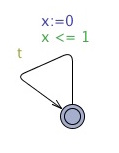
\includegraphics[width=2cm]{./images/tr1.jpg} &   %\hspace{1cm}
 %  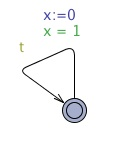
\includegraphics[width=2cm]{./images/tr2.jpg}
 \uppbox[20mm]{LEQ}{./images/tr1} &   %\hspace{1cm}
  \uppbox[20mm]{EQ}{./images/tr2}
\end{tabular}
\\[2mm]
are not \structure{timed-language equivalent}
% \\[2mm]
% \visible<2>{$\pair{(0,t)}$ is not a trace of the TLTS generated by the second system.}

}}
\end{columns}
\end{slide}

%----------------------------------------------------------------------------------
\begin{slide}{Bisimulation}
\small

\begin{block}{Timed bisimulation (between states of timed LTS)}
A relation $R$ is a \structure{timed simulation} iff whenever $s_1 R s_2$, for any action $a$ and delay $d$,
\begin{align*}
s_1\tran{a} s_1'\; & \imp\; \text{there is a transition}\; \; \; s_2 \tran{a} s_2' \e s_1' R s_2'\\
s_1 \tran{d} s_1'\; & \imp\; \text{there is a transition}\; \; \; s_2 \tran{d} s_2' \e s_1' R s_2'
\end{align*}
And a \structure{timed bisimulation} if its converse is also a timed simulation.
\end{block}
\end{slide}

%----------------------------------------------------------------------------------
\begin{slide}{Bisimulation}
\small

\begin{exampleblock}{Example}
\centering
% \wrap{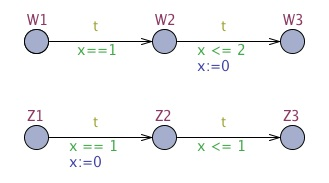
\includegraphics[width=6cm]{./images/bis1.jpg}}
\wrap{\uppbox[50mm]{W1-Z1}{./images/bis1.jpg}}
~~~~
\wrap{W1 bisimilar to Z1?}
\end{exampleblock}

\visible<2>{
\vspace*{-6mm}
\begin{align*}
\pair{\pair{W1,\{x\mapsto 0\}}, \pair{Z1,\{x\mapsto 0\}} } \in R
\end{align*}
where
\[\begin{array}{rlll}
R \; =\;  & \{\pair{\pair{W1,\{x\mapsto d\}}&, \pair{Z1,\{x\mapsto d\}} } &|~d \in \R_0^+\}\; \;   \cup\\
              & \{\pair{\pair{W2,\{x\mapsto d+1\}}&, \pair{Z2,\{x\mapsto d\}} } &|~ d \in \R_0^+\}\; \;  \cup\\
              & \{\pair{\pair{W3,\{x\mapsto d\}}&, \pair{Z3,\{x\mapsto e\}} } &|~d,e \in \R_0^+\}  
\end{array}\]
}


\end{slide}



%----------------------------------------------------------------------------------
\begin{slide}{Untimed Bisimulation}
\small

\begin{block}{Untimed bisimulation}
A relation $R$ is an \structure{untimed simulation} iff whenever $s_1 R s_2$, for any action $a$ and delay $t$,
\begin{align*}
s_1 \tran{a} s_1' \; & \imp\; \text{there is a transition}\; \; \; s_2 \tran{a} s_2' \e s_1' R s_2'\\
s_1 \tran{{\red{d}}} s_1'\; & \imp\; \text{there is a transition}\; \; \; s_2 \tran{{\red{d'}}} s_2' \e s_1' R s_2'
\end{align*}
And it is an \structure{untimed bisimulation} if its converse is also an untimed simulation.
\end{block}
~\\


\alert{Alternatively, it can be defined over a modified LTS in which all delays are abstracted on a 
unique, special transition labelled by $\epsilon$.}
\end{slide}

%----------------------------------------------------------------------------------
\begin{slide}{Untimed Bisimulation}
\small

\doExercise{W1 bisimilar to Z1?}{
\centering
\wrap{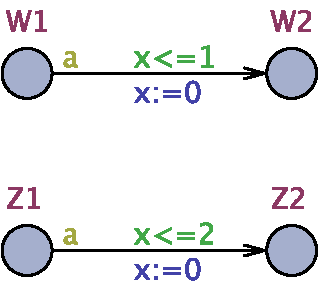
\includegraphics[height=3cm]{./images/bis2}}
% ~~~~
% \wrap{W1 bisimilar to Z1?}
}
\exerciseBack

\visible<2>{
\begin{align*}
\pair{\pair{W1,\{x\mapsto 0\}}, \pair{Z1,\{x\mapsto 0\}} } \in R
\end{align*}
where
\[\begin{array}{r@{~}l@{~}l@{~}l}
R \; =\;  & \{\pair{\pair{W1,\{x\mapsto d\}}&, \pair{Z1,\{x\mapsto d'\}} } &|~0\leq d \leq 1 , 0 \leq d' \leq 2 \}\; \;   \cup\\
      & \ldots
              % & \{\pair{\pair{W1,\{x\mapsto d\}}&, \pair{Z1,\{x\mapsto d'\}} } &|~ d>1, d'>2\}\; \;  \cup\\
              % & \{\pair{\pair{W2,\{x\mapsto d\}}&, \pair{Z2,\{x\mapsto d'\}} } &|~d,d' \in \R_0^+\}  
\end{array}\]
}


\end{slide}
\exerciseAdd

\section{Behavioural Properties}
%----------------------------------------------------------------------------------
\begin{slide}{Properties: expression and satisfaction}
\small
\begin{block}{The satisfaction problem }
Given a \alert{timed automata}, $ta$, and a \structure{property}, $\phi$, show that
\begin{equation*}
\TL{ta} \models \phi
\end{equation*}
\end{block}
~\\

\pause
\begin{itemize}
\item in which logic language shall $\phi$ be specified?
\item how is $\models$ defined?
\end{itemize}
\end{slide}




%----------------------------------------------------------------------------------
\begin{slide}{Expressing properties: \textsc{Uppaal}}
\small

\begin{block}{\textsc{Uppaal} variant of \textsc{CTL}}
\begin{itemize}
\item \structure{state formulae}:  describes individual states in $\TL{ta}$
\item \structure{path formulae}: describes properties of paths in $\TL{ta}$
\end{itemize}
\end{block}

\end{slide}

%----------------------------------------------------------------------------------
\begin{slide}{Expressing properties: \textsc{Uppaal}}
\small

\begin{block}{State formulae}
\vspace*{-4mm}
\begin{align*}
% \Pi\; ::=\; & \Ac \Boxc\, \Psi\, \mid\, \Ac\Diamondc\, \Psi\, \mid\, \Ec \Boxc\, \Psi\, \mid\, \Ec \Diamondc\, \Psi\, \mid\, \Phi \leadsto  \Psi\
% % \tag{path}
% \\[2mm]
\Psi\; ::=\; & ta.\ell ~|~ g_c ~|~ {\transp{g_d}} ~|~ \texttt{deadlock} ~|~
  \texttt{not~}\Psi ~|~ \Psi \texttt{ or }\Psi ~|~ \Psi \texttt{ and }\Psi ~|~
  \Psi \texttt{ imply }\Psi
  % \tag{state}
\end{align*}

Any expression which can be evaluated to a boolean value for a state (typically involving the 
\alert{clock constraints} used for guards and invariants and similar constraints over integer variables):
\vspace*{-6mm}
\begin{center}
\texttt{x >= 8}, \texttt{i == 8 and x < 2}, ...
\end{center}
Additionally,
\begin{itemize}
\item \structure{$ta.\ell$} which tests \alert{current location}:  $(\ell, \eta) \models ta.\ell$ \\
provided $(\ell, \eta)$ is a state in $\TL{ta}$
\item \structure{$\texttt{deadlock}$}: $(\ell, \eta) \models \forall_{d \in \R_0^+} .\, \text{there is no transition from} \; \pair{\ell,\eta+d}$ 
\end{itemize}

\end{block}

\end{slide}



\begin{slide}{Exercises}
  \centering
  \uppbox[7cm]{Lamp}{./images/Lamp}

  \doExercise{Write a state formula}{
  \vspace*{-8mm}
  \begin{enumerate}
    \item The lamp is \texttt{low}
    \item Not \texttt{off} and $y>25$
    \item If it is \texttt{low} or \texttt{bright}, then $y\leq 3600$
  \end{enumerate}
  }
  
\end{slide}

%----------------------------------------------------------------------------------
\begin{slide}{Expressing properties: \textsc{Uppaal}}
\small

\newcommand{\Boxc}{\alert{\Box}}
\newcommand{\Diamondc}{\alert{\Diamond}}
\newcommand{\Ac}{\structure{A}}
\newcommand{\Ec}{\structure{E}}

\begin{block}{Path formulae}
\begin{align*}
\Pi\; ::=\; & \Ac \Boxc\, \Psi\, \mid\, \Ac\Diamondc\, \Psi\, \mid\, \Ec \Boxc\, \Psi\, \mid\, \Ec \Diamondc\, \Psi\, \mid\, \Phi \leadsto  \Psi\
% \tag{path}
% \\[2mm]
% \Psi\; ::=\; & ta.\ell ~|~ g_c ~|~ {\transp{g_d}} ~|~ \texttt{deadlock} ~|~
%   \texttt{not~}\Psi ~|~ \Psi \texttt{ or }\Psi ~|~ \Psi \texttt{ and }\Psi ~|~
%   \Psi \texttt{ imply }\Psi
%   \tag{state}
\end{align*}

where
\begin{itemize}
\item \structure{$A$, $E$} quantify (universally and existentially, resp.) over \structure{paths}
\item \alert{$\Box$, $\Diamond$} quantify (universally and existentially, resp.) over \alert{states in a path}
\end{itemize}
also notice that

\vspace*{-3mm}
\begin{align*}
 \Phi \leadsto  \Psi\; \abv\; \Ac \Boxc\, (\Phi \imp \Ac \Diamondc\, \Psi)
\end{align*}
\end{block}

\end{slide}




% \uppbox[2.8cm]{\Large $A \Box\, \varphi$}{./images/AA.jpg}~~
% \uppbox[2.8cm]{$A \Diamond \, \varphi$}{./images/AE.jpg}


\begin{slide}{Expressing properties: \textsc{Uppaal}}
\small \centering

\uppbox[2.8cm]{\Large $A \Box\, \varphi$}{./images/AA.jpg}~
\uppbox[2.8cm]{\Large $A \Diamond \, \varphi$}{./images/AE.jpg}~~~~~
\uppbox[2.8cm]{\Large $E \Box\, \varphi$}{./images/EA.jpg}~
\uppbox[2.8cm]{\Large $E \Diamond\, \varphi$}{./images/EE.jpg}

\end{slide}

%----------------------------------------------------------------------------------
% \begin{slide}{Expressing properties: \textsc{Uppaal}}
% \small \centering

% ~\\
% \begin{tabular}{cc}
%   \Large $A \Box\, \varphi$ & \Large $A \Diamond \, \varphi$ \\
%  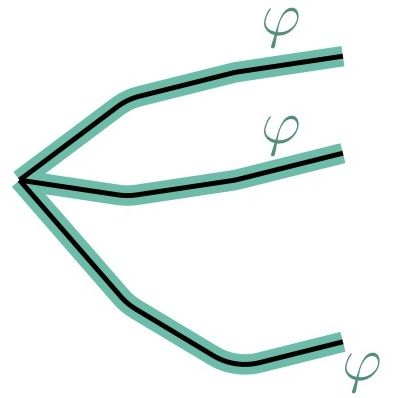
\includegraphics[width=2.8cm]{./images/AA.jpg} &
%  \hspace{1cm} 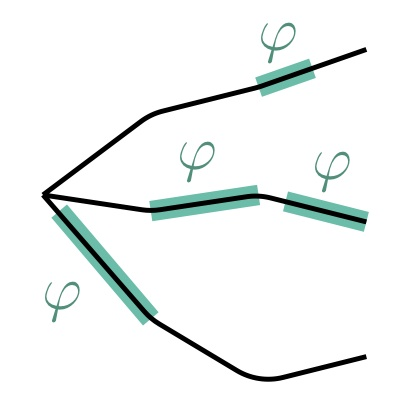
\includegraphics[width=2.8cm]{./images/AE.jpg}
% \end{tabular}

% ~\\[2mm]

% % \begin{block}{$E \Box\, \varphi$ and $E \Diamond\, \varphi$}
% \begin{tabular}{cc}
%   \Large $E \Box\, \varphi$ & \Large $E \Diamond\, \varphi$ \\
%  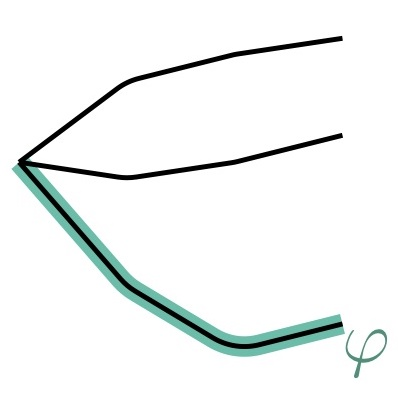
\includegraphics[width=2.8cm]{./images/EA.jpg} &   \hspace{1cm} 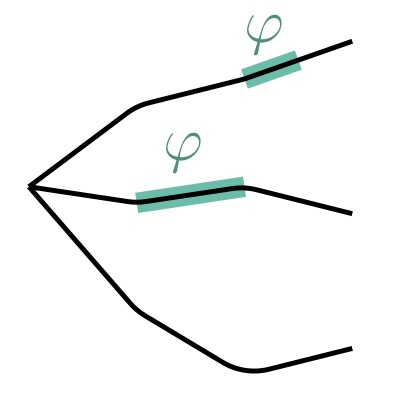
\includegraphics[width=2.8cm]{./images/EE.jpg}
% \end{tabular}
% % \end{block}
% \end{slide}

%----------------------------------------------------------------------------------
\begin{slide}{Expressing properties: \textsc{Uppaal}}
\small \centering

\uppbox[5cm]{\Large $\varphi\, \leadsto\, \psi$}{./images/LeadsTo.jpg}

% \begin{block}{$\varphi\, \leadsto\, \psi$}
% \begin{center}
%   \Large $\varphi\, \leadsto\, \psi$ \\
%  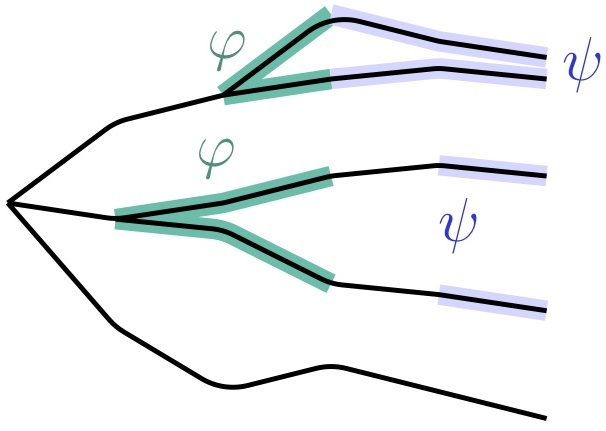
\includegraphics[width=5cm]{./images/LeadsTo.jpg} 
%  \end{center}
% \end{block}

\begin{exampleblock}{Example}
  If a message is sent, it will eventually be received -- $\texttt{send(m)} \leadsto \texttt{received(m)}$
\end{exampleblock}

\end{slide}

%----------------------------------------------------------------------------------
\begin{slide}{Reachability properties}
\small

\begin{block}{$E \Diamond\, \phi$}
\structure{Is there a path starting at the initial state, such that a state formula $\phi$ is eventually satisfied?}

\begin{itemize}
\item  Often used to perform sanity checks  on a model:
\begin{itemize}
\item \alert{is it possible for a sender to send a message?}
 \item \alert{can a message possibly be received?}
 \item ...
 \end{itemize}
 \item  Do not by themselves guarantee the correctness of the protocol (i.e. \alert{that any message is eventually delivered}), 
but they validate the basic behavior of the model.
 \end{itemize}
\end{block}

\end{slide}


%----------------------------------------------------------------------------------
\begin{slide}{Safety properties}
\small

\begin{block}{$A \Box\, \phi$ and $E \Box\, \phi$}
\vspace{5mm}
\structure{Something bad will never happen}\\
 or \structure{something bad will possibly never happen}
\vspace{5mm}

Examples\\
\begin{itemize}
\item \alert{In a nuclear power plant the temperature of the core is always (invariantly) under a certain threshold}.
\item \alert{In a game a safe state is one in which we can still win, ie, will possibly not loose}.
\end{itemize}

In Uppaal these properties are formulated positively: something good is invariantly true.
\end{block}

\end{slide}

%----------------------------------------------------------------------------------
\begin{slide}{Liveness properties}
\small

\begin{block}{$A \Diamond\, \phi$ and $\phi\, \leadsto \, \psi$}
\vspace{5mm}
\structure{Something good will \emph{eventually happen}}\\
 or \structure{if \emph{something} happens, then \emph{something else} will eventually happen!}
\vspace{5mm}

Examples\\
\begin{itemize}
\item \alert{When pressing the on button, then eventually the television should turn on}.
\item \alert{In a communication protocol, any message that has been sent should eventually be received}.
\end{itemize}

\end{block}

\end{slide}



%\end{document}




\begin{slide}{Exercise: worker, hammer, nail - revisited}
\small
\begin{columns}
\col[.45]{
  \centering
  ~\\[2mm]
  % Requires \usepackage{graphicx}
  % ~~~~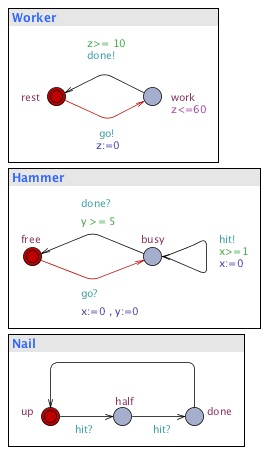
\includegraphics[width=45mm]{./images/WHN.jpg}
  \uppbox[30mm]{Worker}{./images/Worker.pdf}\\[2mm]
  \uppbox[30mm]{Hammer}{./images/Hammer.pdf}\\[2mm]
  \uppbox[30mm]{Nail}{./images/Nail.pdf}\\
}
\col[.54]{
  \doExercise{Write properties and explain them}{
    \vspace*{-4mm}
    \begin{enumerate}
      \item Using $E\Diamond$
      \item Using $E\Box$
      \item Using $A\Diamond$
      \item Using $A\Box$
      \item Using $\leadsto$
    \end{enumerate}
    (Practice in UPPAAL)
  }
}
\end{columns}
\end{slide}


\begin{slide}{Exercise: write formulas}
  \centering
  \uppbox[4.5cm]{Lamp}{./images/Lamp}

  \vspace*{-2mm}
  \doExercise{Write formulas, and say which ones are true}{
    \vspace*{-8mm}
    % \begin{multicols}{2}
    \begin{enumerate}
      \item The lamp can become bright;
      \item The lamp will eventually become bright;
      \item The lamp can never be on for more than 3600s;
      \item It is possible to never turn on the lamp;
      \item Whenever the light is bright, the clock $y$ is non-zero;
      \item Whenever the light is bright, it will eventually become off.
    \end{enumerate}
    % \end{multicols}
    }
\end{slide}



\section{Examples: proving mutual exclusion}
% \section{Case-study: proving mutual exclusion}



%----------------------------------------------------------------------------------
\begin{slide}{The train gate example (1/2)}
\small

\begin{columns}

\col[0.35]{
\begin{center}
% \includegraphics[width=4cm]{./images/tg1.jpg}
\uppbox[5cm]{Train(id)}{./images/Train} 
\end{center}
}

\col[0.65]{
\begin{itemize}
\item \visible<2>{\texttt{E<> Train(0).Cross}}
\\ \structure{(Train 0 can reach the cross)}
\item \visible<2>{\texttt{E<> Train(0).Cross and Train(1).Stop}}
\\ \structure{(Train 0 can be crossing bridge while Train 1 is waiting to cross)}
\item \visible<2>{\texttt{E<> Train(0).Cross and}
\\ \texttt{~~~~~~~(forall (i:id-t)}
\\ \texttt{~~~~~~~~~~~~i != 0 imply Train(i).Stop)}}
\\ \structure{(Train 0 can cross bridge while the other trains are waiting to cross)}
\end{itemize}
}

\end{columns}
\end{slide}

%----------------------------------------------------------------------------------
\begin{slide}{The train gate example (2/2)}
\small

\begin{columns}

\col[0.35]{
\begin{center}
% \includegraphics[width=4cm]{./images/tg1.jpg}
\uppbox[5cm]{Train(id)}{./images/Train} 
\end{center}
}

\col[0.65]{
\begin{itemize}
\item \visible<2>{\texttt{A[] Gate.list[N] == 0}}
\\ \structure{There can never be N elements in the queue}
\item \visible<2>{\texttt{A[] forall (i:id-t) forall (j:id-t) Train(i).Cross \&\& Train(j).Cross imply i == j}}
\\ \structure{There is never more than one train crossing the bridge}
\item \visible<2>{\texttt{Train(1).Appr --> Train(1).Cross}}
\\ \structure{Whenever a train approaches the bridge, it will eventually cross}
\item \visible<2>{\texttt{A[] not deadlock}}
\\ \structure{The system is deadlock-free}
\end{itemize}
}
\end{columns}

\end{slide}



%%----------------------------------------------------------------------------------
%\begin{slide}{The train gate example}
%\small
%
%\begin{center}
%\includegraphics[width=5cm]{./images/tg2.jpg} 
%\end{center}
%
%\begin{itemize}
%\item Note the use of parameters and the select clause on transitions
%\item Programming ...
%\end{itemize}
%
%\end{slide}





%%----------------------------------------------------------------------------------
%\begin{slide}{Demo}
%\small
%
%
%\begin{itemize}
%\item The \alert{train gate} case study (included in the \textsc{Uppaal} distribution).
%\end{itemize}
%
%\end{slide}
%
%


%----------------------------------------------------------------------------------
\begin{slide}{Mutual exclusion}
\small

\begin{block}{Properties}
\begin{itemize}
\item \structure{mutual exclusion}: \alert{no two processes are in their critical sections at the same time}
\item \structure{deadlock freedom}: \alert{if some process is trying to access its critical section, then 
eventually some process (not necessarily the same) will be in its critical section; similarly for exiting the critical section}
\end{itemize}
\end{block}
\end{slide}

%%----------------------------------------------------------------------------------
\begin{slide}{Mutual exclusion}
\small


\begin{block}{The Problem}
\begin{itemize}
\item 
Dijkstra's original asynchronous algorithm (1965) requires, for $n$ processes to be controlled,
$\mathcal{O}(n)$ read-write registers and $\mathcal{O}(n)$ operations.
\item
This result is a theoretical limit (proved by Lynch and Shavit in 1992) which compromises scalability.
\end{itemize}
\end{block}
\pause
\fbox{but it can be overcome by introducing specific \structure{timing constraints}}
%\end{block}

\begin{block}{Two \emph{timed} algorithms:}
\begin{itemize}
\item  \structure{Fisher's protocol} (included in the \textsc{Uppaal} distribution)
\item  \structure{Lamport's protocol}
\end{itemize}
\end{block}
\end{slide}


%----------------------------------------------------------------------------------
\begin{slide}{Fisher's algorithm}
\small

\begin{block}{The algorithm}
\begin{align*}
\mathsf{repeat} & \\
& \mathsf{repeat}  \\
&  \hspace{1cm} \mathsf{await} \; id = 0\\
& \hspace{1cm} id := i\\
& \hspace{1cm}  \mathsf{delay}(k)\\ 
& \mathsf{until}\; id=i  \\
& \text{\emph{(critical section)}}\\
& id := 0\\
\mathsf{forever} &
\end{align*}
\end{block}
\end{slide}


%%----------------------------------------------------------------------------------
%\begin{slide}{Alur \& Taubenfeld's algorithm}
%\small
%
%\begin{block}{The algorithm}
%\begin{align*}
%\mathsf{repeat} & \\
%& s:\;  x:=i\\
%&\mathsf{await}\, (y = 0)\\
%& y := i\\
%& \mathsf{if}\;  x \neq i \; \mathsf{then}\,\\
%&  \hspace{1cm} \mathsf{delay}(2d); \\
%&  \hspace{1cm}  \mathsf{if}\; y \neq i \; \mathsf{then}\,\mathsf{goto}\, s; \\
%&  \hspace{1cm}  \mathsf{await}\, (\neg z)\\
%&  \mathsf{else}\, z:= true;\\
%& \text{\emph{(critical section)}}\\
%& z := false\\
%& \mathsf{if}\;  y = i \; \mathsf{then}\; y:=0;\\
%\mathsf{forever} &
%\end{align*}
%\end{block}
%\end{slide}


%----------------------------------------------------------------------------------
\begin{slide}{Fisher's algorithm}
\small
\begin{block}{Comments}
\begin{itemize}
\item One shared read/write register (the variable $id$)
\item Behaviour depends crucially on the value for $k$ --- the \structure{time delay}
\item Constant $k$ should be \alert{larger than the longest time that a process may take to perform a step while trying to get access to its critical section} 
\item This choice guarantees that whenever process $i$ finds $id = i$ on testing the loop guard it can enter safely ist critical section: \alert{all} other processes are out of the loop or with their index in $id$ overwritten by $i$.
\end{itemize}
\end{block}
\end{slide}

%----------------------------------------------------------------------------------
\begin{slide}{Fisher's algorithm in \textsc{Uppaal}}
\small
\centering

% 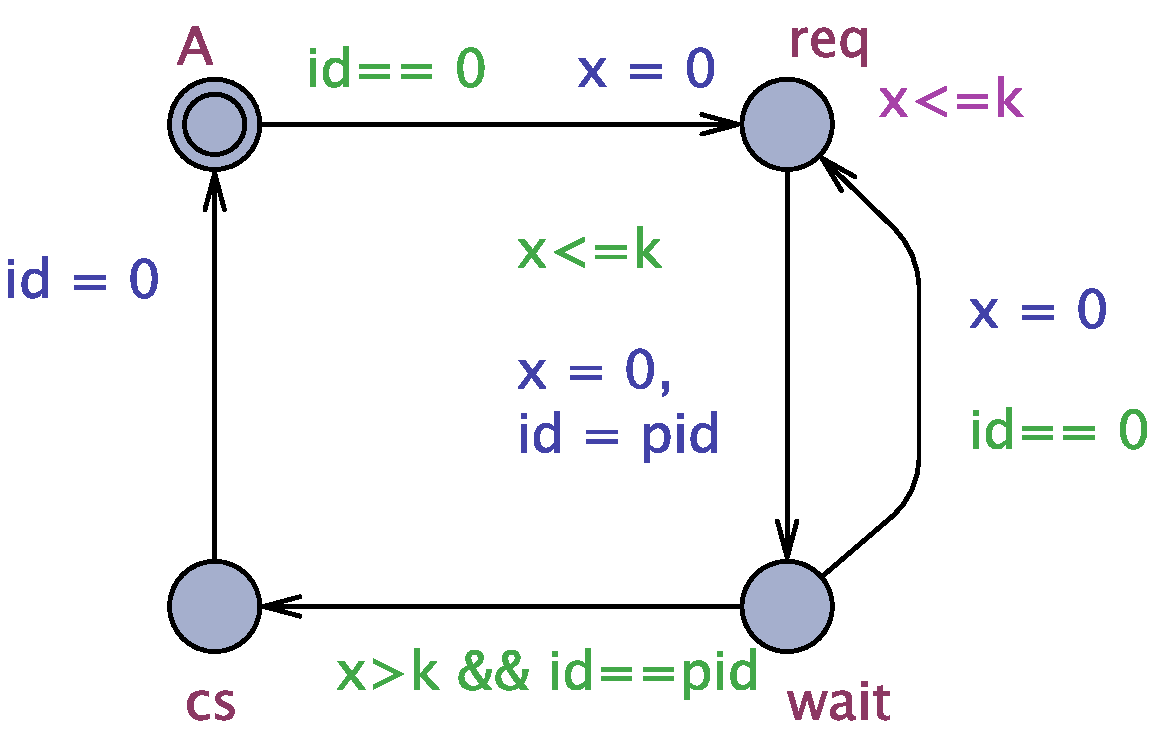
\includegraphics[width=6cm]{./images/P.pdf} 
\uppbox[5cm]{Fisher}{./images/P.pdf} 
%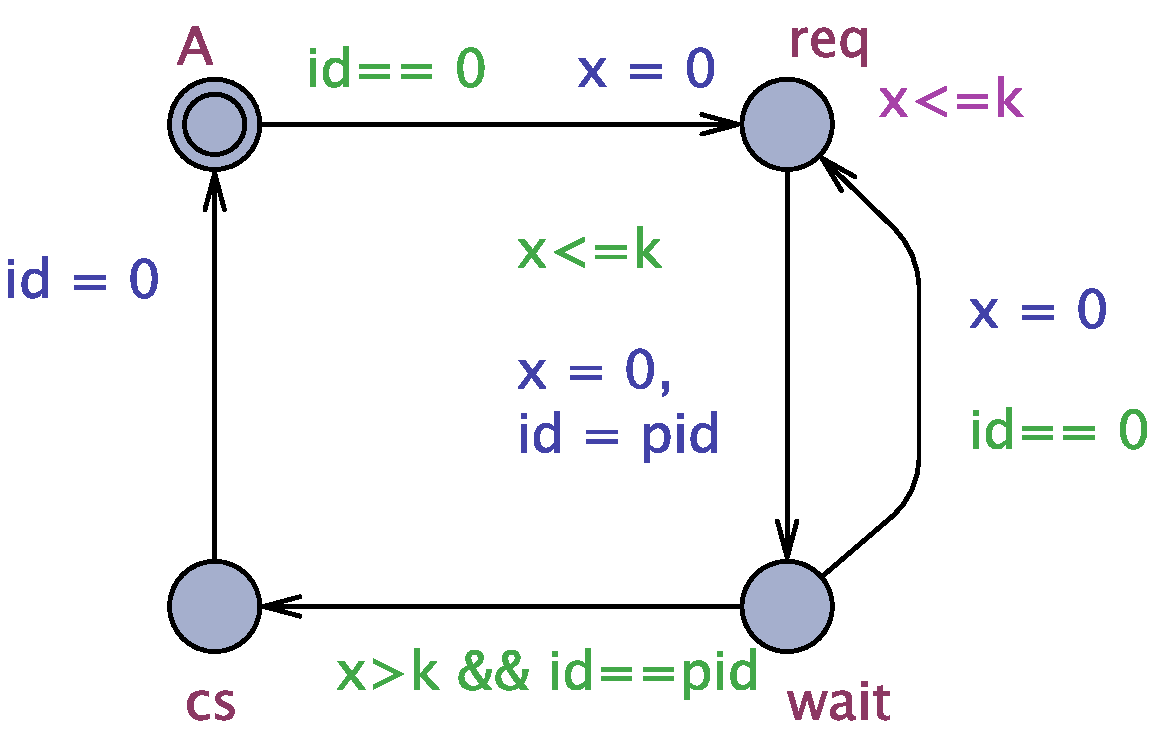
\includegraphics[width=1.1\textwidth]{./images/P.pdf} 


\begin{itemize}
\item Each process uses a local clock $x$ to guarantee that the upper bound between between its successive steps, while
trying to access the critical section, is $k$ (cf. \alert{invariant} in state $req$).
\item \alert{Invariant} in state $req$ establishes $k$ as such an upper bound
\item \alert{Guard} in transition from $wait$ to $cs$ ensures the correct delay before entering the critical section
\end{itemize}
\end{slide}

%----------------------------------------------------------------------------------
\begin{frame}[fragile]{Fisher's algorithm in \textsc{Uppaal}}
\small

\begin{block}{Properties}
%\includegraphics[width=12cm]{./images/ficher2.jpg} 
\begin{lstlisting}[emph={[2]forall,not}]
% P(1) requests access => it will eventually wait
P(1).req -> P(1).wait
% the algorithm is deadlock-free
A[] not deadlock
% mutual exclusion invariant
A[] forall (i:int[1,6]) forall (j:int[1,6])
   P(i).cs && P(j).cs imply i == j  
\end{lstlisting}
\end{block}

\begin{itemize}
\item The algorithm is \alert{deadlock-free}
\item It ensures  mutual exclusion if the correct timing constraints. 
\item ... but it is critically sensible to  small violations of such constraints: for example, replacing $x > k$ by 
$x \geq k$ in the transition leading to $cs$ compromises both \alert{mutual exclusion} and \alert{liveness}.
\end{itemize}
\end{frame}


%----------------------------------------------------------------------------------
\begin{slide}{Lamport's algorithm}
\small

\begin{block}{The algorithm}
\begin{align*}
\mathsf{start}: \; \;  &  a := i\\
& \mathsf{if}\; b \neq 0\; \mathsf{then\; goto\; start}\\
& b := i \\
& \mathsf{if}\; a \neq i\; \mathsf{then\; delay}(k)\\
& \hspace{12mm} \mathsf{else} \; \mathsf{if}\; b \neq i\; \mathsf{then\; goto\; start}\\
& \text{\emph{(critical section)}}\\
& b := 0
\end{align*}
\end{block}
\end{slide}

%----------------------------------------------------------------------------------
\begin{slide}{Lamport's algorithm}
\small
\begin{block}{Comments}
\begin{itemize}
\item Two shared read/write registers (variables $a$ and $b$)
\item Avoids \alert{forced waiting} when no other processes are requiring access to their critical sections
\end{itemize}
\end{block}
\end{slide}


%----------------------------------------------------------------------------------
\begin{slide}{Lamport's algorithm in \textsc{Uppaal}}
\small
\centering

% \begin{center}
% 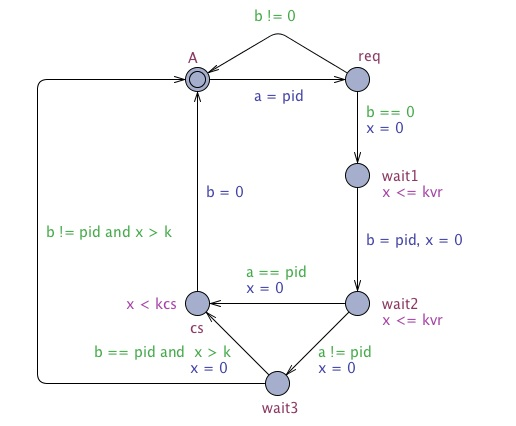
\includegraphics[width=9cm]{./images/lamport.jpg} 
\uppbox[80mm]{Lamport}{./images/lamport.jpg} 
% \end{center}

~\\[-6mm]

\hspace*{-130mm}%
\begin{tikzpicture}[remember picture, overlay]
  \node[draw=red,circle,very thick] at (242pt,125pt){~~~~};
  \node[draw=red,circle,very thick] at (242pt,69pt){~~~~};
  \node[draw=red,circle,very thick] at (159pt,51pt){~~~~};
  \node[draw=red,circle,very thick] at (128pt,76pt){~~~~};
  \node[draw=red,circle,very thick] at (132pt,107pt){~~~~};
\end{tikzpicture}

\end{slide}


%----------------------------------------------------------------------------------
\begin{slide}{Lamport's algorithm}
\small
\begin{columns}[T]

\col[0.43]{
\begin{block}{Model time constants:}
\begin{itemize}
\item \structure{$k$} --- time delay
\item \structure{$kvr$} --- max bound for register access
\item \structure{$kcs$} --- max bound for permanence in critical section 
\end{itemize}
Typically
\vspace{-10mm}
\begin{center}
\fbox{$k\; \geq \; kvr + kcs$}
\end{center}
\end{block}
}


\col[0.55]{
\begin{block}{Experiments}
\centering
\begin{tabular}{|l|c|c|c|c|}
\hline
& $k$ & $kvr$ & $kcs$ & verified? \\
\hline
Mutual Exclusion & 4 & 1 & 1 & Yes\\
Mutual Exclusion & 2 & 1 & 1 & Yes\\
Mutual Exclusion & 1 & 1 & 1 & No\\
No deadlock & 4 & 1 & 1 & Yes\\
No deadlock & 2 & 1 & 1 & Yes\\
No deadlock  & 1 & 1 & 1 & Yes\\
\hline
\end{tabular}
\end{block}
}
\end{columns}
\end{slide}


\end{document}
